\documentclass[c, compress, ngerman,  presentation, final, xcolor=svgnames]{beamer}

% standard packages
\usepackage[utf8]{inputenc}
\usepackage{times}
\usepackage[T1]{fontenc}
\usepackage{eurosym, babel}
\usepackage{amsmath}

% \usepackage{listings}
% \usepackage{multimedia, fancybox}
% \usepackage{calc, amssymb, amsmath, amsfonts}
% \usepackage{pstricks, pst-bar}
% \usepackage{graphicx}
% \usepackage{color}
% \usepackage{caption3} % load caption package kernel first


% ---------- for example pages ----------------
\usepackage{tikz}
\usetikzlibrary{arrows}
\tikzstyle{block}=[draw opacity=0.7,line width=1.4cm]
% ---------------------------------------------


% ---------- various options ----------------
\usepackage[small]{caption}
\DeclareCaptionOption{parskip}[]{} % disable "parskip" caption option
\setbeamercovered{transparent} % enable semi transparent bullet points
% ---------------------------------------------


% ---------- color and theme settings ----------------
\usetheme{Darmstadt}
\usecolortheme[named=SteelBlue]{structure}

\usefonttheme[onlylarge]{structurebold}
\setbeamerfont*{frametitle}{size=\normalsize,series=\bfseries}

%\setbeamertemplate{items}[ball] % round numberings and bullets
%\setbeamertemplate{blocks}[rounded][shadow=true] %rounded boxes with shadows
\setbeamertemplate{navigation symbols}{} %hide navigation symbols
% ---------------------------------------------


% ---------- Footnote ----------------
\setbeamertemplate{footline} {
\begin{beamercolorbox}[wd=0.5\textwidth,ht=3ex,dp=1.5ex,leftskip=.5em,rightskip=.5em]{author in head/foot}%
\usebeamerfont{author in head/foot}%
\hfill \insertshortauthor%
\end{beamercolorbox}%
\vspace*{-4.5ex}\hspace*{0.5\textwidth}%
\begin{beamercolorbox}[wd=0.5\textwidth,ht=3ex,dp=1.5ex,left,leftskip=.5em]
{title in head/foot}%
\usebeamerfont{title in head/foot}%
\insertshorttitle \hfill \hfill \hfill \hfill \insertframenumber%
\end{beamercolorbox} }
% ---------------------------------------------


% ---------- Author, Title, etc. ----------------
\title[] {PRIMO}
\subtitle[]{PRobabilistic Inference MOdules}
\author[]{Manuel Baum, Denis John, \\ Lukas Kettenbach, Maximilian Koch}
\institute[]{Bielefeld University}
\date{\today}
% ---------------------------------------------


% ---------- document start ----------------
\begin{document}

\maketitle

%\begin{frame}{Table of Contents}{}
%	\tableofcontents%[pausesections]
%\end{frame}

%\AtBeginSection{\begin{frame}<beamer>{Gliederung} \tableofcontents[currentsection, currentsubsection] \end{frame}}

%\input{010_example}
\section{Introduction}

\begin{frame}
\frametitle{Introduction}
\Large\textbf{Idea}
\begin{itemize}
\item probabilistic inference modules for Python
\item library which offers well known probabilistic (graphical) models like Bayesian or temporal networks
\item variety of inference algorithms
\end{itemize}

\Large\textbf{Download/Documentation/Installation Guide}
\begin{itemize}
\item \url{github.com/mbaumBielefeld/PRIMO}
\item \url{github.com/mbaumBielefeld/PRIMO/wiki}
\end{itemize}

\end{frame}

\begin{frame}
\frametitle{Structure}
\Large\textbf{PRIMO/}
\begin{itemize}
\item doc/
\item examples/
\item primo/
\begin{itemize}
\item core/ $\rightarrow$ BayesNet.py, Node.py, DynamicBayesNet.py, ...
\item decision/ $\rightarrow$ DecisionNode.py, UtilityNode.py, ...
\item reasoning/ $\rightarrow$ DiscreteNode.py, density/, MCMC.py, ...
\item tests/
\item utils/ $\rightarrow$ XMLBIF.py
\end{itemize}
\item setup.py 
\end{itemize}
\end{frame}
\section{Dynamic Bayesian Networks}
\subsection{Definition}
\begin{frame}
%\frametitle{Dynamic Bayesian Networks}
\begin{definition}
        A DBN is a pair $(B_0, B_{\rightarrow})$, where $B_0$ is a Bayesian network over $\chi^{(0)}$ representing the initial distribution, and $B_{\rightarrow}$ is a 2-TBN for the process. For any desired time span $T \geq 0$, the distribution over $\chi^{(0:T)}$ is defined as a unrolled Bayesian network, where, for any $i=1,...,n$:
        \begin{itemize}
        \item the structure and CPDs of $X_i^{(0)}$ are the same as those for $X_i$ in $B_0$,
        \item the structure and CPDs of $X_i^{(t)}$ for $ t \geq 0 $ are the same as those for $X_i^{'}$ in $B_\rightarrow$.
        \end{itemize}
\end{definition}
\end{frame}

\subsection{Example}
\begin{frame}
%\frametitle{Example}
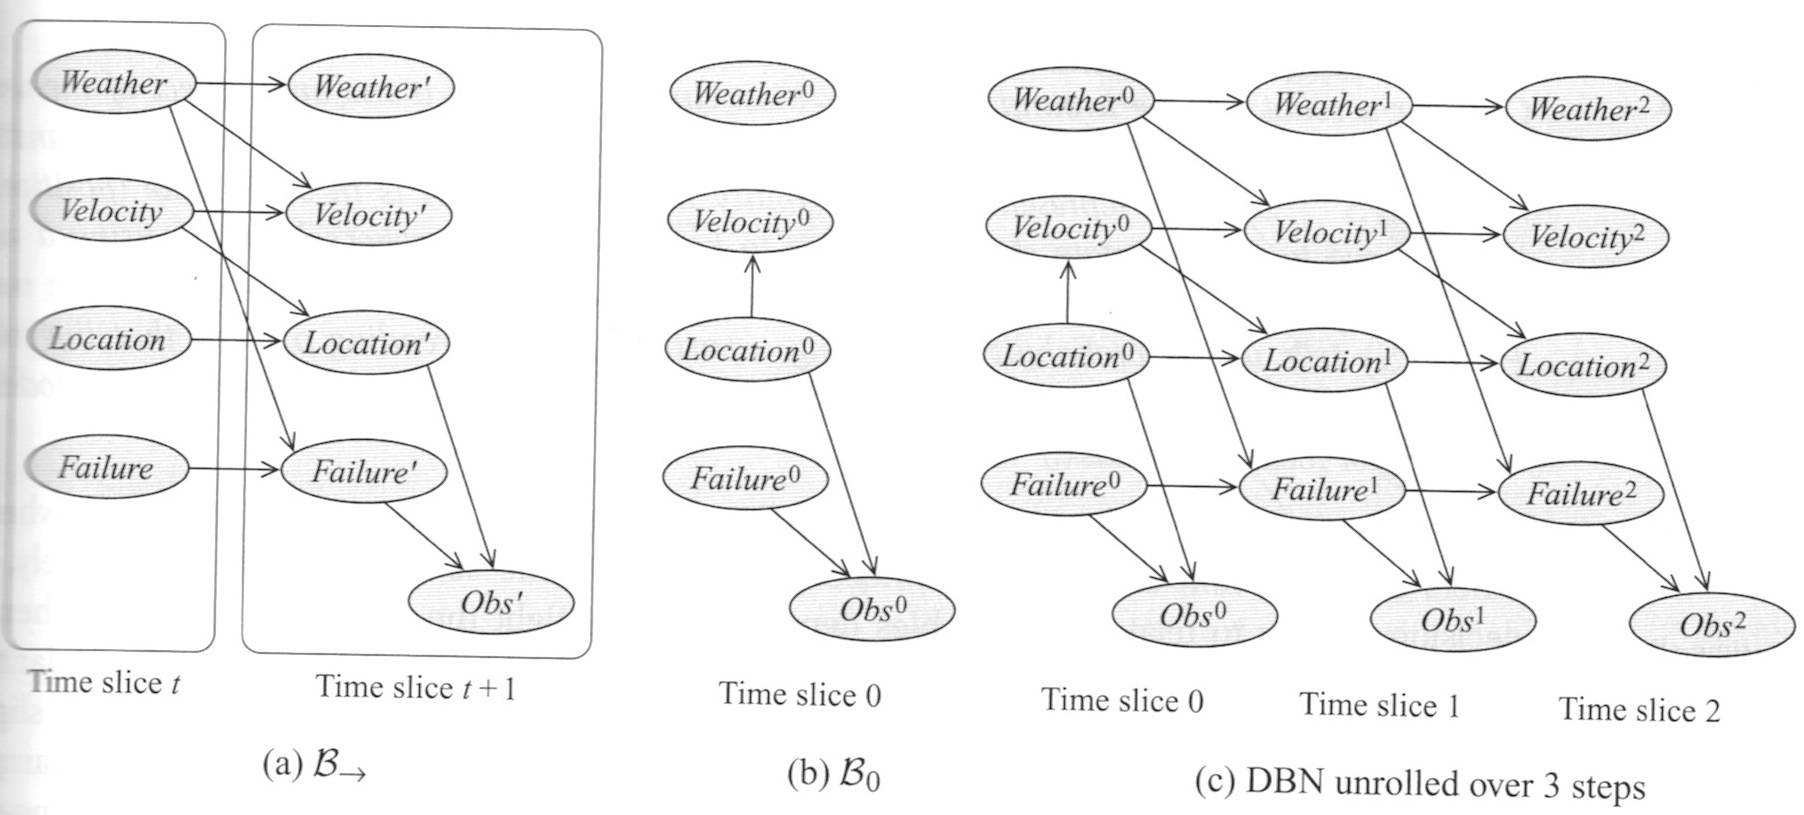
\includegraphics[width=1\textwidth]{figures/dbn}
\end{frame}

\subsection{Inference}

\begin{frame}
\frametitle{Exact Inference}
\begin{itemize}
\item We can use standard inference algorithms (e.g. variable elimination)
\item Problem I: run inference on larger an larger networks over time
\item Problem II: maintain our entire history of observations indefinitely
\item Solution/workaround: use approximate inference
\end{itemize}
\end{frame}

\begin{frame}
\frametitle{Approximate Inference}
\begin{itemize}
\item We can use some kind of Likelihood Weighting
\item Two modifications:
\begin{enumerate}
\item run all samples together through the DBN, one slice at a time
\item focus the set of samples on the high-probability regions of the state space
\end{enumerate}
\item Particle Filter:
\begin{enumerate}
\item Each sample is propagated forward by sampling the next state value $x_{t+1}$ given the current value $x_t$ for the sample
\item Each sample is weighted by the likelihood it assigns to the new evidence $P(e_{t+1}|x_{t+1})$
\item The population is \textit{resampled} to generate a new population of $N$ samples. Each new sample is selected from the current population; the probability that a particular sample is selected is proportional to its weight.
\end{enumerate}
\end{itemize}
\end{frame}

\begin{frame}
\frametitle{Algorithm}
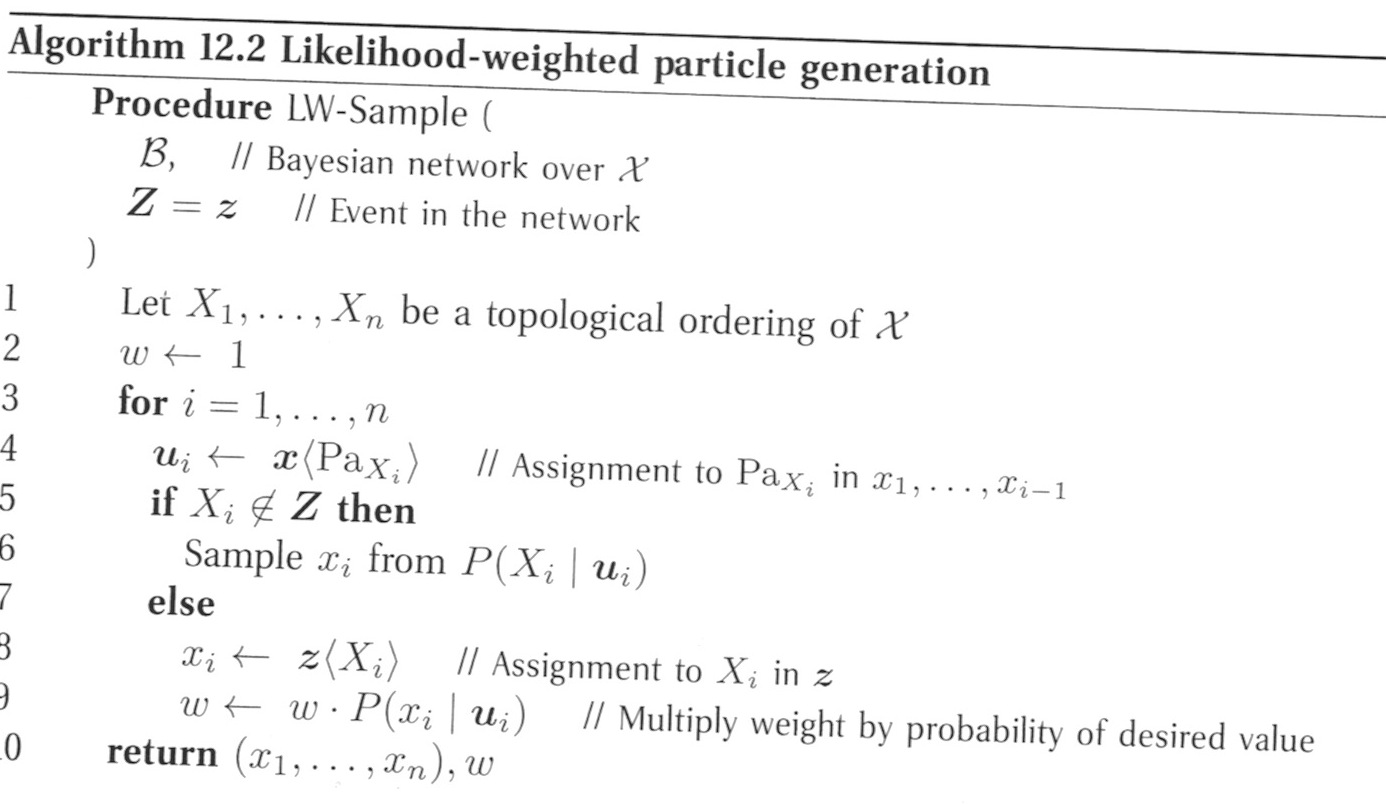
\includegraphics[width=1\textwidth]{figures/lwalgsimple}
\end{frame}

\begin{frame}
\frametitle{Algorithm}
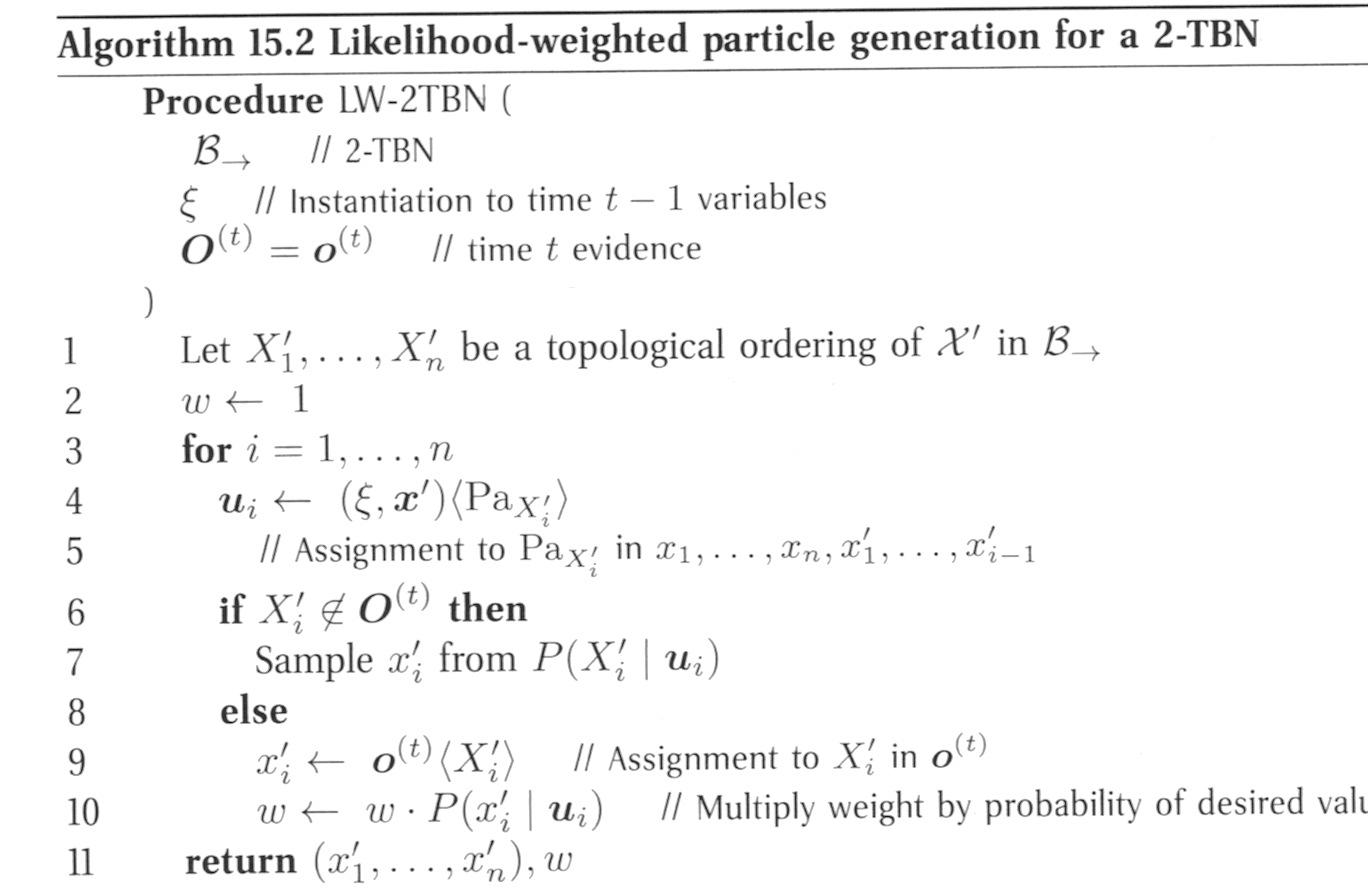
\includegraphics[width=1\textwidth]{figures/lwalg}
\end{frame}

\begin{frame}
\frametitle{Algorithm}
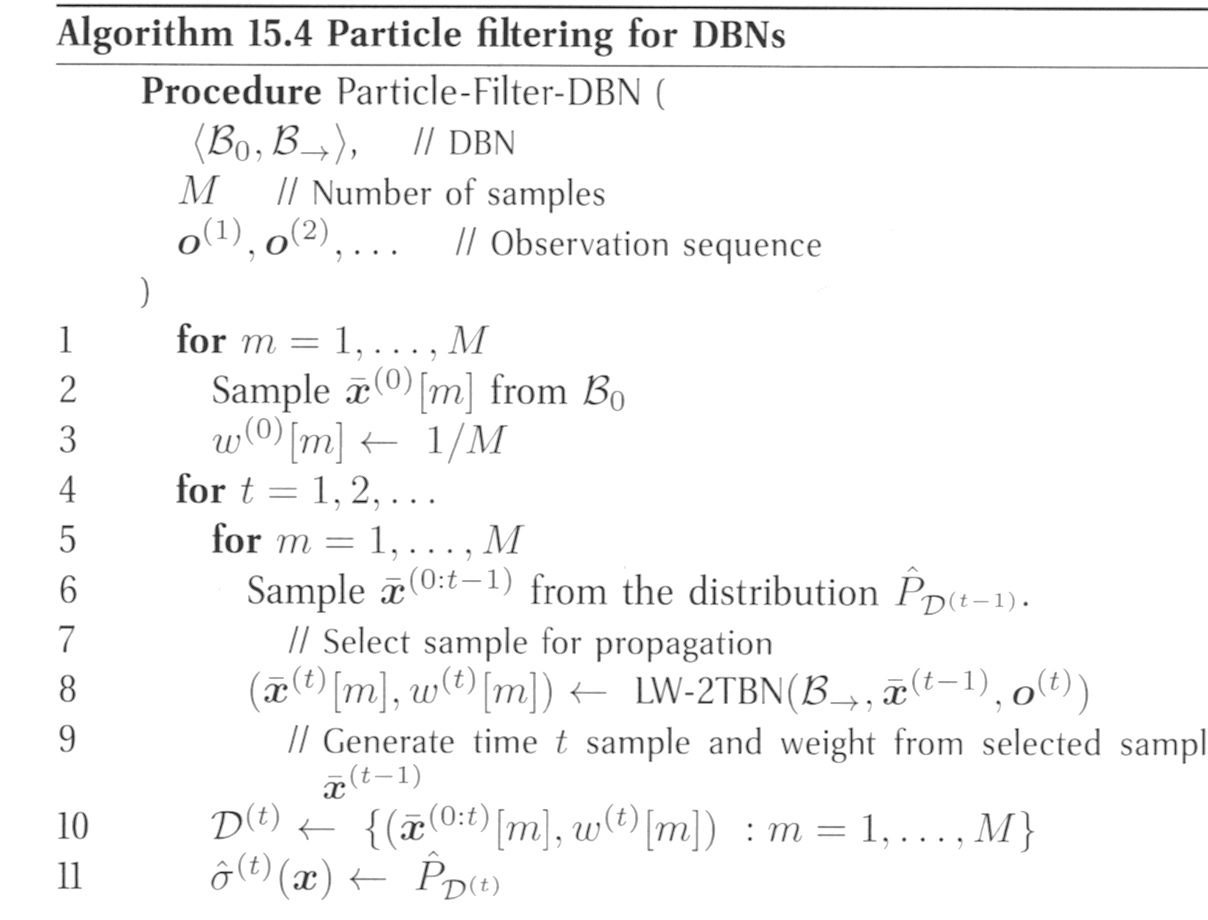
\includegraphics[width=.8\textwidth]{figures/pfalg}
\end{frame}

\subsection{Structure}
\begin{frame}
\frametitle{Algorithm}
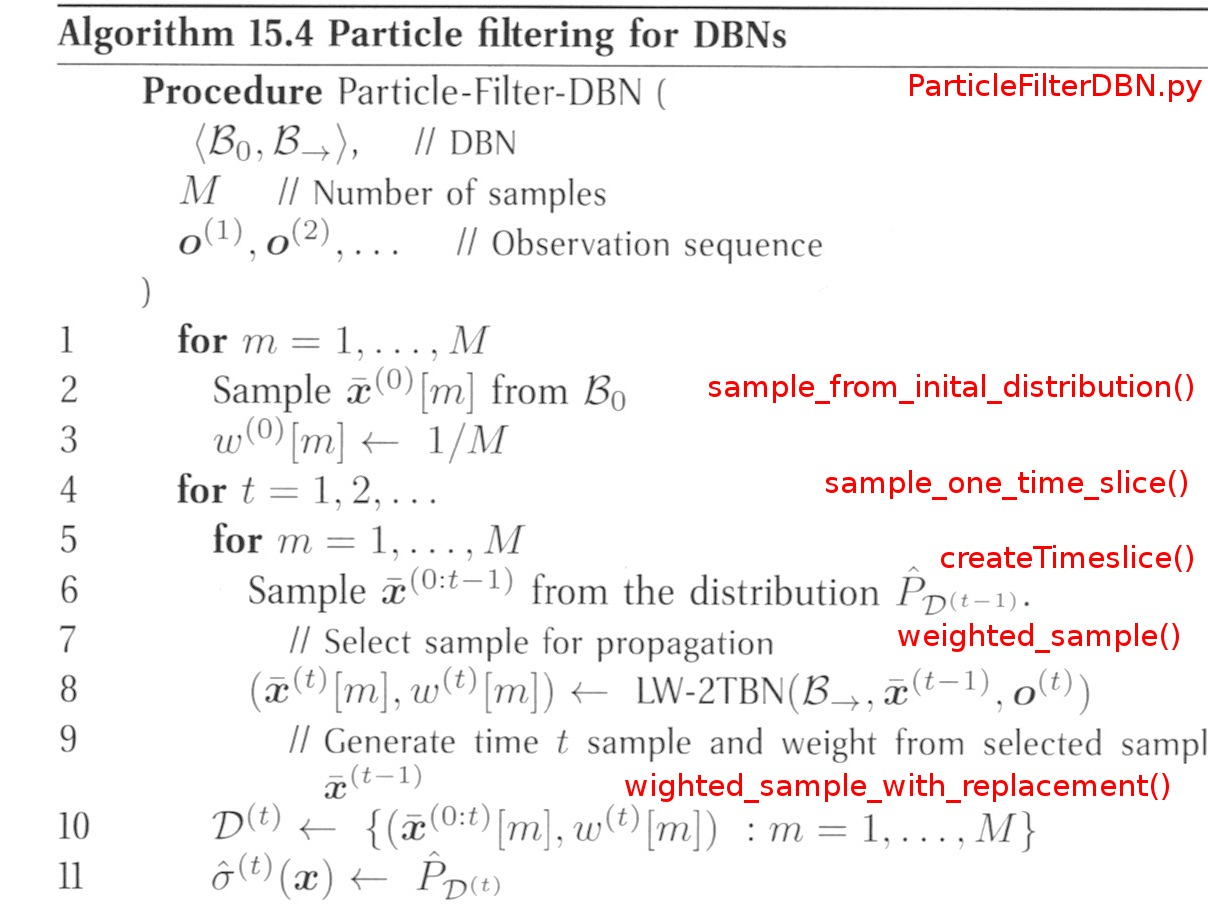
\includegraphics[width=.8\textwidth]{figures/pfalg_code}
\end{frame}

\begin{frame}
\frametitle{Files}
\Large\textbf{PRIMO/primo/}
\begin{itemize}
	\item core/
	\begin{itemize}
		\item DynamicBayesNet.py
		\item TowTBN.py (create\_timeslice())
	\end{itemize}
	\item reasoning/particlebased/
	\begin{itemize}
		\item ParticleFilterDBN.py (sample\_from\_inital\_distribution(), wighted\_sample\_with\_replacement(), ...)
	\end{itemize}
	\item tests/
	\begin{itemize}
		\item DynamicBayesNet\_test.py
		\item XMLBIF\_test.py
	\end{itemize}
	\item utils/
	\begin{itemize}
		\item XMLBIF.py
	\end{itemize}
\end{itemize}
\end{frame}

\subsection{Literature}
\begin{frame}
\begin{itemize}
\item \textsc{Stuart Russell and Peter Norvig} \\ Artificial Intelligence: A Modern Approach
\item \textsc{Daphne Koller and Nir Friedman} \\ Probabilistic Graphical Models: Principles and Techniques
\end{itemize}
\end{frame}

\section{Factor Trees}
% Task
% Factor Elimination
% Performance depends on elimination order
% Factor tree with messages
% tree building

\subsection{Task Description}


\begin{frame}
\frametitle{Task Description}
\begin{columns}
\column{.4\textwidth}
\begin{itemize}
\item Exact inference
\item Use elimination trees
\item Prior Marginal, Posterior Marginal \& PoE
\end{itemize}
\column{0.6\textwidth}
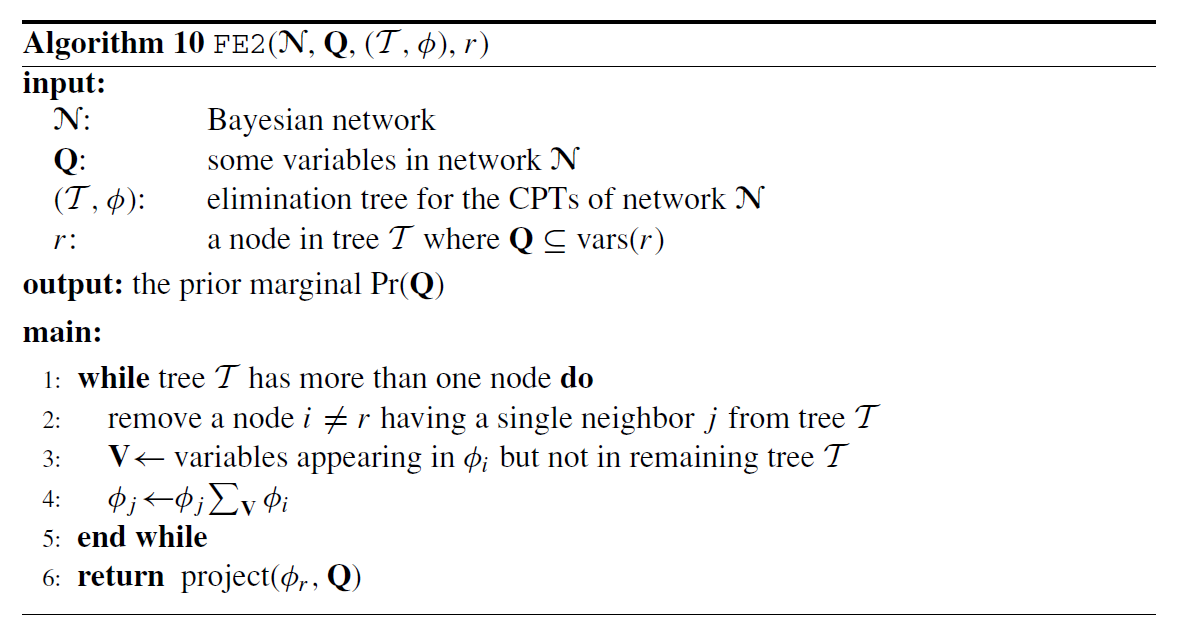
\includegraphics[width=.8\textwidth]{figures/algo10}
\end{columns}
\end{frame}




\subsection{Factor Elimination}



\subsection{Elimination Trees}

\subsection{Building Strategies}


\subsection{Literature}

\begin{frame}
\frametitle{Literature}
\begin{itemize}
\item Modeling and Reasoning with Bayesian Networks , Adnan Darwiche 
\end{itemize}
\end{frame}

\begin{frame}
\textbf{Thank you for your attention!}
\end{frame}


\section{manu}
\section{max}


\end{document}
